\documentclass[10pt]{article}
%%%%%%%%%%%%%%%%%%%%%%%%%%%%%%%%%%%%%%%%
\usepackage{amsmath}
\usepackage{verbatim}
\usepackage[usenames,dvipsnames]{color}
\usepackage{ulem}
\usepackage{setspace}
\usepackage{lscape}
\usepackage{longtable}
\usepackage[top=1.25in,bottom=1.5in,left=1in,right=1.5in,landscape]{geometry}
\usepackage{graphicx}
\usepackage{epstopdf}
\usepackage[usenames,dvipsnames]{pstricks}
\usepackage{epsfig}
\usepackage{pstricks-add}
\usepackage{pst-node}
\usepackage{fancyhdr}
\usepackage[absolute,showboxes]{textpos}

%TCIDATA{OutputFilter=LATEX.DLL}
%TCIDATA{Version=5.00.0.2552}
%TCIDATA{<META NAME="SaveForMode" CONTENT="1">}
%TCIDATA{Created=Thursday, August 28, 2003 13:38:44}
%TCIDATA{LastRevised=Thursday, August 14, 2008 15:20:27}
%TCIDATA{<META NAME="GraphicsSave" CONTENT="32">}
%TCIDATA{<META NAME="DocumentShell" CONTENT="Standard LaTeX\Blank - Standard LaTeX Article">}
%TCIDATA{Language=American English}
%TCIDATA{CSTFile=LaTeX article (bright).cst}

\setcounter{MaxMatrixCols}{10}

\newenvironment{proof}[1][Proof]{\noindent\textbf{#1.} }{\ \rule{0.5em}{0.5em}}
\setlength{\columnsep}{.2in}

\renewcommand{\labelitemii}{$\cdot$}

\pagestyle{fancy} \fancyhead{} \fancyfoot{} \rfoot{} \lfoot{}

\newcommand{\slide}[2]{
\begin{textblock}{11}(0,0)
\textcolor{Black}{\textbf{\huge \rule{0pt}{1in} \raisebox{.2in}{#1}}}
\end{textblock}
\begin{Large} \noindent
#2
\end{Large}
\vfill \pagebreak}

\setlength{\TPHorizModule}{1in}
\setlength{\TPVertModule}{1in}
\textblockcolour{Yellow}
\renewcommand{\headrulewidth}{0pt}



\begin{document}
\onehalfspacing 

\lfoot{Introduction} \rfoot{Economic Growth}

\slide{Fact 1}{\textbf{There is enormous variation in per capita income across economies. The poorest countries have per capita incomes that are less than 5 percent of per capita income in the richest countries.}

\vspace{.25in}\noindent Several notes:
\begin{itemize}
	\item Income per capita (or GDP per capita) is not the sole measure of what is good: but it's a useful summary statistic
	\item Income per capita ignores distribution of income within a country
	\item Comparing income per capita across countries is not trivial
	\begin{itemize}
		\item You have to convert between currencies
		\item Countries have different relative prices for goods
		\item What is the ``right'' way to value haircuts, apples, or cars across countries?
	\end{itemize}
\end{itemize}
}

\slide{Rich Countries}{
\begin{tabular}{lccccc}\hline
 & GDP per capita & GDP per worker & LF Part. Rate & Avg. Growth & Years to \\
Country & 2008 & 2008 & 2008 & 1960-2008 &  Double \\ \hline \hline
United States  & \$43,326 & \$84,771 & 0.51 & 1.6 & 43 \\
Japan & 33,735 & 64,778 & 0.52 & 3.4 & 21 \\
France & 31,980 & 69,910 & 0.46 & 2.2 & 30 \\
United Kingdom & 35,345 & 70,008 & 0.51 & 1.9 & 36 \\
Spain & 28,958 & 57,786 & 0.50 & 2.7 & 26 \\ \hline
\end{tabular}
}

\slide{Poor Countries}{
\begin{tabular}{lccccc}\hline
 & GDP per capita & GDP per worker & LF Part. Rate & Avg. Growth & Years to \\
Country & 2008 & 2008 & 2008 & 1960-2008 &  Double \\ \hline \hline
China & 6,415 & 10,938 & 0.59 & 5.6 & 13 \\
India & 3,078 & 7,801 & 0.39 & 3.0 & 24 \\
Nigeria & 1,963 & 6,106 & 0.32 & 0.6 & 114 \\
Uganda & 1,122 & 2,604 & 0.43 & 1.3 & 52 \\ \hline
\end{tabular}
}

\slide{Growth Miracles}{
\begin{tabular}{lccccc}\hline
 & GDP per capita & GDP per worker & LF Part. Rate & Avg. Growth & Years to \\
Country & 2008 & 2008 & 2008 & 1960-2008 &  Double \\ \hline \hline
Hong Kong & 37,834 & 70,940 & 0.53 & 4.3 & 16 \\
Singapore & 49,987 & 92,634 & 0.54 & 4.1 & 17 \\
Taiwan & 29,645 & 62,610 & 0.47 & 5.1 & 14 \\
South Korea & 25,539 & 50,988 & 0.50 & 4.5 & 16 \\ \hline
\end{tabular}
}

\slide{Growth Disasters}{
\begin{tabular}{lccccc}\hline
 & GDP per capita & GDP per worker & LF Part. Rate & Avg. Growth & Years to \\
Country & 2008 & 2008 & 2008 & 1960-2008 &  Double \\ \hline \hline
Venezuela & 9,762 & 21,439 & 0.46 & -0.1 & -627 \\
Haiti & 1,403 & 3,164 & 0.44 & -0.4 & -168 \\
Madagascar & 810 & 1,656 & 0.49 & -0.1 & -488 \\
Zimbabwe & 135 & 343 & 0.40 & -1.5 & -47 \\  \hline
\end{tabular}
}

\slide{Distribution of Population by GDP per Worker, 2008}{
\begin{center}
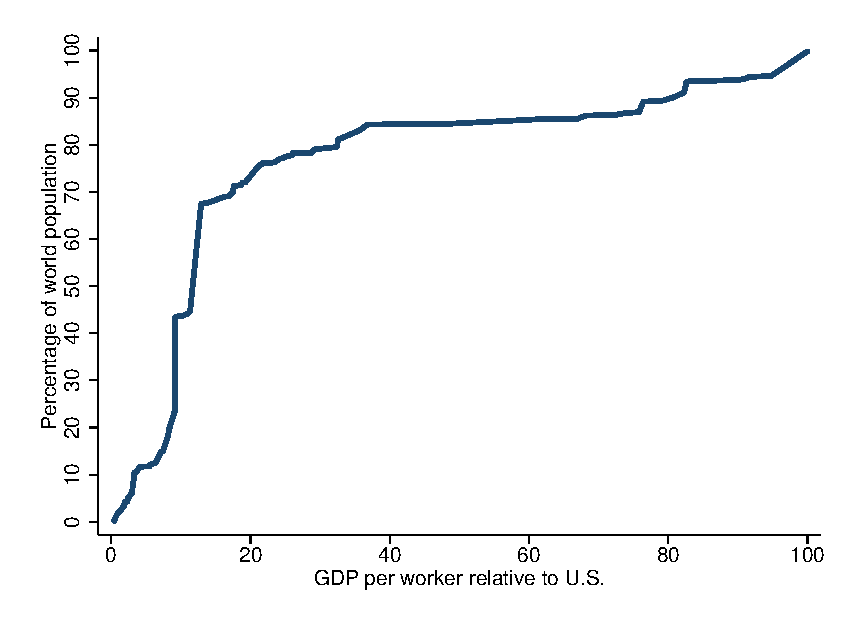
\includegraphics[scale=1.2]{figure_1_1.eps}
\end{center}
}

\slide{World Population by GDP per Worker, 1960 and 2008}{
\begin{center}
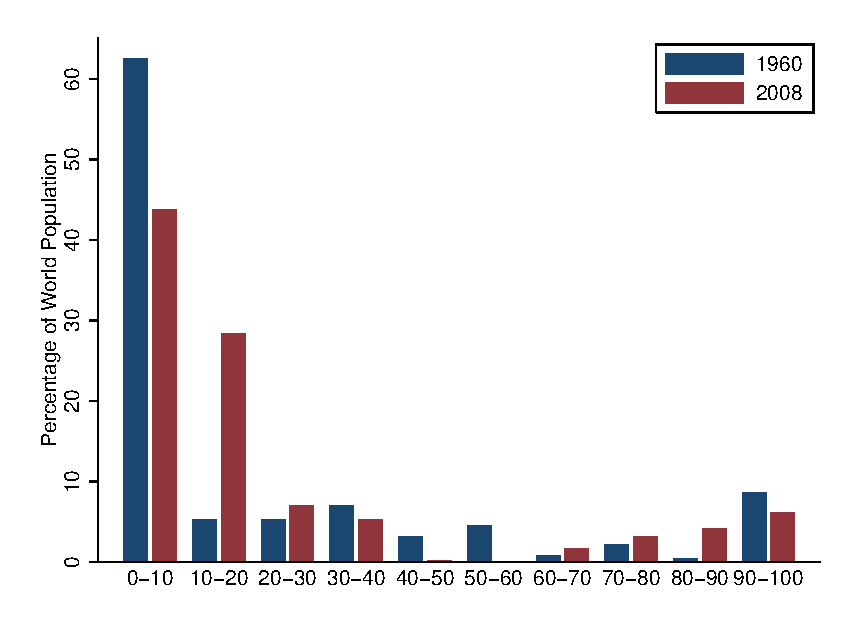
\includegraphics[scale=1.2]{figure_1_2.eps}
\end{center}
}

\slide{Fact 2}{\textbf{Rates of economic growth vary substantially across countries.}

\vspace{.25in}\noindent Notes:
\begin{itemize}
	\item We will try to distinguish whether these are long-term differences or just transitional differences
	\item If they are long-term, then eventually some countries will be infinitely rich compared to others
	\item We think most differences are transitional
\end{itemize}
}

\slide{Fact 3}{\textbf{Growth rates are not generally constant over time. For the world as a whole, growth rates were close to zero over most of history but have increased sharply in the twentieth century. For individual countries, growth rates also change over time.}

\vspace{.25in}\noindent Note:
\begin{itemize}
	\item The big changes in growth rates over history are from pre-Industrial Revolution (close to 0\% growth) to modern times (roughly 1.85\% growth per year for developed countries)
	\item The big changes in growth rates within countries tend to be as they transition from poor to rich (e.g. Japan or China), after which growth slows down.
\end{itemize}

}

\slide{World GDP per Capita Growth Rates}{
\begin{center}
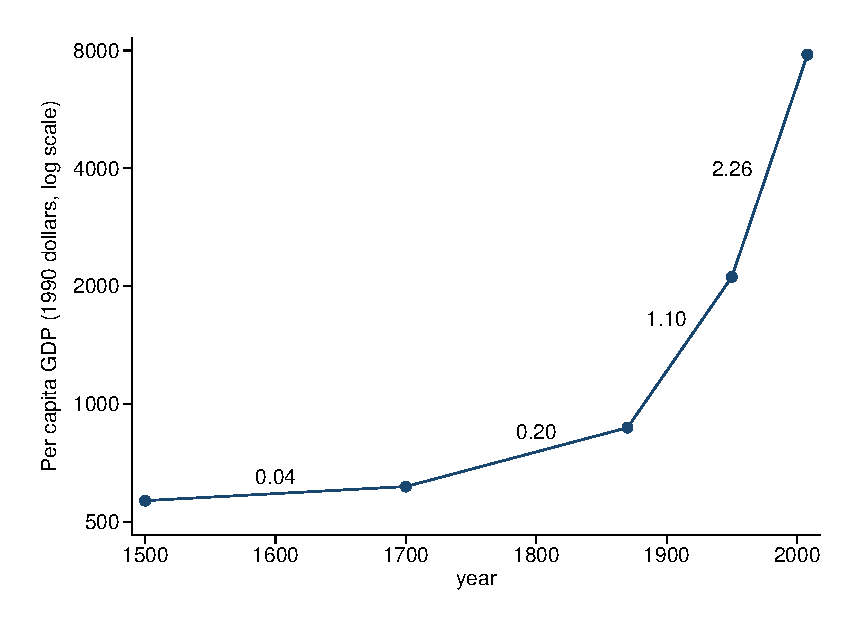
\includegraphics[scale=1.2]{figure_1_3.eps}
\end{center}
}

\slide{Fact 4}{\textbf{A country's relative position in the world distribution of per capita incomes is not immutable. Countries can go from being ``poor'' to being ``rich'', and vice versa.}

\vspace{.25in}\noindent Notes:
\begin{itemize}
	\item The ``growth disasters'' in the table were all very well off in 1960 compared to East Asia. Now they are well behind
	\item The ``growth miracles'' in the table were though, in 1960, to be on the path to starvation and destitution. 
	\item What are the sources of these movements in rankings?
\end{itemize}
}

\slide{Fact 5}{\textbf{In the U.S. over the last century,
\begin{itemize}
	\item The real rate of return on capital, $r$, shows no trend upward or downward
	\item The shares of income devoted to capital, $rK/Y$, and labor, $wL/Y$, show no trend; and
	\item The average growth rate of output per person has been positive and relatively constant over time - that is, the United States exhibits steady, sustained per capita income growth.
\end{itemize}}

\vspace{.25in}\noindent Notes:
\begin{itemize}
	\item ``Kaldor facts''
	\item Questions about the first two, are they really true over long periods of time?
	\item These facts will drive us to look at a specific pattern of growth - the \textit{balanced growth path}
\end{itemize}

}

\slide{Growth in U.S. GDP per capita}{
\begin{center}
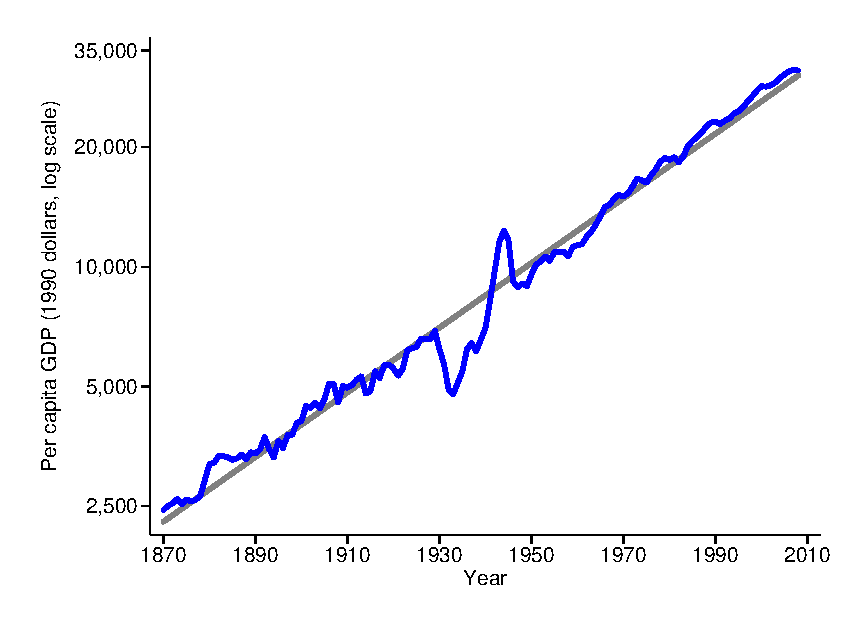
\includegraphics[scale=1.2]{figure_1_4.eps}
\end{center}
}

\slide{Fact 6}{\textbf{Growth in output and growth in the volume of international trade are closely related.}

\vspace{.25in}\noindent Notes:
\begin{itemize}
	\item Growth in trade is associated with growth in output, but not necessarily level of trade (Japan does not actually trade much, but is rich)
	\item Rapid growth in trade is no necessarily just growth in exports from East Asia (China and Korea also import a lot more than they used to)
\end{itemize}
}

\slide{Growth in Trade and Growth in Output}{
\begin{center}
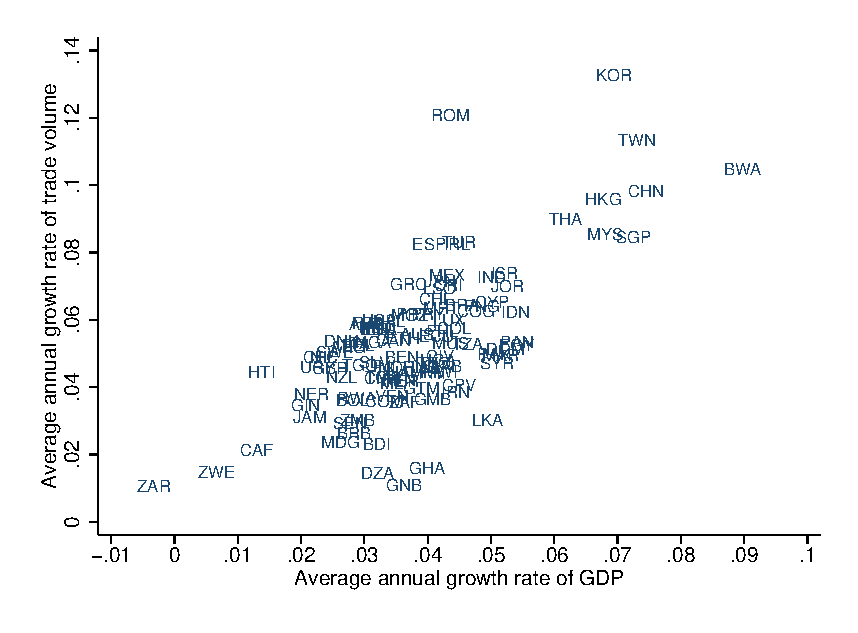
\includegraphics[scale=1.2]{figure_1_5.eps}
\end{center}
}

\slide{Fact 7}{\textbf{Both skilled and unskilled workers tend to migrate from poor to rich countries or regions.}

\vspace{.25in}\noindent Notes:
\begin{itemize}
	\item Implies that return to both kinds of labor is higher in developed countries
	\item Shouldn't scarcity in poor countries imply a large premium to skilled workers?
\end{itemize}
}

\slide{Big Questions}{\textbf{Why are some countries so rich and others so poor?}

\vspace{.25in}\noindent Answers?
\begin{itemize}
	\item Level differences
	\item Different levels of human capital
	\item Different institutions supporting innovation/technology adoption/entrepreneurship
\end{itemize}

}

\slide{Big Questions}{\textbf{What is the engine of growth?}

\vspace{.25in}\noindent Answers?
\begin{itemize}
	\item Technological progress - new goods, or better versions of old goods
	\item Not accumulation of more physical or human capital - those cannot sustain growth
	\item Ultimately technological progress will rely on population - more people, more ideas
\end{itemize}
}

\slide{Big Questions}{\textbf{What creates growth miracles in some countries?}

\vspace{.25in}\noindent Answers?
\begin{itemize}
	\item Reversing what made them poor
	\item Changing institutions to foster technology adoption (copying?)
	\item Changing institutions to create larger markets (trade, internal markets) to support innovation/adoption
\end{itemize}
}

\end{document}